% CS 3000 Midterm 2 Note Sheet — Portrait, 3 columns per side
% Compile on Overleaf: pdflatex (default engine)
\documentclass[9pt]{extarticle}
\usepackage[portrait, margin=0.3in, top=0.25in, bottom=0.25in]{geometry}
\usepackage{multicol}
\usepackage{tcolorbox}
\usepackage{booktabs}
\usepackage{amsmath}
\usepackage{amssymb}
\usepackage{tikz}
\usepackage{microtype}
\usetikzlibrary{arrows.meta,positioning,calc}
\tcbuselibrary{skins}

% No enumitem — use plain list spacing instead
\makeatletter
\renewcommand{\itemize}{\list{\textbullet}{%
  \setlength{\itemsep}{0pt}\setlength{\topsep}{1pt}%
  \setlength{\parsep}{0pt}\setlength{\partopsep}{0pt}%
  \setlength{\leftmargin}{1em}}}
\renewcommand{\enumerate}{\list{\arabic{enumi}.}{%
  \usecounter{enumi}%
  \setlength{\itemsep}{0pt}\setlength{\topsep}{1pt}%
  \setlength{\parsep}{0pt}\setlength{\partopsep}{0pt}%
  \setlength{\leftmargin}{1.2em}}}
\makeatother

\setlength{\parindent}{0pt}
\setlength{\parskip}{0pt}
\setlength{\columnsep}{4pt}
\setlength{\columnseprule}{0.2pt}

% Colors
\definecolor{darkgreen} {RGB}{26,92,53}
\definecolor{darkblue}  {RGB}{26,58,110}
\definecolor{darkpurple}{RGB}{61,26,110}
\definecolor{darkred}   {RGB}{110,26,26}
\definecolor{darkteal}  {RGB}{26,92,90}
\definecolor{darkamber} {RGB}{92,62,26}
\definecolor{lightblue} {RGB}{216,232,252}
\definecolor{lightgreen}{RGB}{208,240,218}
\definecolor{lightorange}{RGB}{253,232,208}
\definecolor{lightyellow}{RGB}{255,251,235}
\definecolor{lightmint} {RGB}{235,255,240}
\definecolor{lightred}  {RGB}{255,235,235}
\definecolor{lightgray} {RGB}{245,245,242}

\tcbset{
  nb/.style={fonttitle=\bfseries\footnotesize\sffamily, coltitle=white,
    boxrule=0.4pt, arc=1.5pt, left=2pt, right=2pt, top=0pt, bottom=1pt,
    toptitle=1pt, bottomtitle=1pt, boxsep=0pt},
  green/.style ={nb,colback=white,colframe=darkgreen, colbacktitle=darkgreen},
  blue/.style  ={nb,colback=white,colframe=darkblue,  colbacktitle=darkblue},
  purple/.style={nb,colback=white,colframe=darkpurple,colbacktitle=darkpurple},
  red/.style   ={nb,colback=white,colframe=darkred,   colbacktitle=darkred},
  teal/.style  ={nb,colback=white,colframe=darkteal,  colbacktitle=darkteal},
  amber/.style ={nb,colback=white,colframe=darkamber, colbacktitle=darkamber},
}

\newcommand{\yb}[1]{\vspace{1pt}\noindent\colorbox{lightyellow}{\parbox{\dimexpr\linewidth-2\fboxsep}{\footnotesize\sffamily #1}}\vspace{1pt}}
\newcommand{\gb}[1]{\vspace{1pt}\noindent\colorbox{lightmint}  {\parbox{\dimexpr\linewidth-2\fboxsep}{\footnotesize\sffamily #1}}\vspace{1pt}}
\newcommand{\rb}[1]{\vspace{1pt}\noindent\colorbox{lightred}   {\parbox{\dimexpr\linewidth-2\fboxsep}{\footnotesize\sffamily #1}}\vspace{1pt}}
\newcommand{\grb}[1]{\vspace{1pt}\noindent\colorbox{lightgray} {\parbox{\dimexpr\linewidth-2\fboxsep}{\footnotesize\sffamily #1}}\vspace{1pt}}
\newcommand{\cd}[1]{{\fontsize{7}{8.5}\selectfont\ttfamily\noindent #1}}
\newcommand{\kv}[2]{\noindent{\footnotesize\sffamily\textbf{#1}}\;{\small #2}\par\vspace{1pt}}

\begin{document}
\small

%%=============================================================
%% SIDE 1
%%=============================================================
\noindent{\centering\normalsize\bfseries\sffamily
  CS 3000 MIDTERM 2 --- SIDE 1: Greedy Algorithms \& Graph Traversals\par}
\vspace{2pt}
\begin{multicols}{3}

\begin{tcolorbox}[blue,title=Key Terms]
\small
\textbf{Graph} $G{=}(V,E)$: vertices $V$, edges $E$. \textit{Directed} = one-way; \textit{undirected} = bidirectional.

\textbf{Weight} $w(e)$: cost on an edge. Unweighted = all costs 1.

\textbf{DAG}: Directed Acyclic Graph --- no directed cycles. Required for topo sort. Every tree is a DAG.

\textbf{SCC}: Strongly Connected Component --- maximal set where every vertex reaches every other via directed paths. In a DAG, each node is its own SCC.

\textbf{Condensation}: contract each SCC to one node $\Rightarrow$ always a DAG.

\textbf{Topological order}: linear order s.t.\ every edge $(u{\to}v)$ has $u$ before $v$. Exists iff DAG. Unique iff Kahn's always has exactly 1 source.

\textbf{Relaxation}: if $\mathrm{dist}[u]{+}w(u,v)<\mathrm{dist}[v]$, update $\mathrm{dist}[v]$. Core of Dijkstra and Bellman-Ford.

\textbf{disc/fin}: DFS clock starts at 1, $+1$ each discover or finish. $\mathrm{fin}[v]$ set when DFS fully backtracks out of $v$. Max fin $=2|V|$.

\textbf{Greedy stays ahead}: induction --- show greedy's running measure $\geq$ OPT's at every step.

\textbf{Exchange arg}: take OPT, find first diff from greedy, swap to match greedy, show cost $\not\uparrow$, repeat.

\textbf{Product state space}: two agents $\Rightarrow$ vertices = pairs $(u,v)$, up to $|V|^2$ nodes. Dijkstra still valid if all weights $\geq 0$.
\end{tcolorbox}

\vspace{3pt}
\begin{tcolorbox}[green,title=GreedyJump --- Algorithm]
\small
\kv{Heuristic:}{jump to farthest stone $\leq$10 ft away}
\kv{Optimizes:}{(1) min jumps \; (2) max unused stones \; (3) max avg jump}
\kv{Does NOT:}{min longest jump; min avg jump length}

\vspace{2pt}
\cd{A=[0]; i=0; d(n+1)=inf\hfill\% sentinel\\
while i < n:\\
\quad j = i\\
\quad while d(j)-d(i) <= 10: j++\hfill\% overshoot\\
\quad append j-1 to A\hfill\% step back\\
\quad i = j-1\\
return A}

\vspace{2pt}Inner loop exits when $j$ is first stone \textit{too far}, so $j{-}1$ is farthest reachable.

\vspace{2pt}\textbf{Example} $d{=}[0,3,8,11,19,25,28]$:

\cd{i=0: j stops at 3 (11>10) -> stone 2 (d=8)\\
i=2: j stops at 4 (11>10) -> stone 3 (d=11)\\
i=3: j stops at 5 (14>10) -> stone 4 (d=19)\\
i=4: j stops at 7 (inf)   -> stone 6 (d=28)\\
A = [0, 2, 3, 4, 6]}
\end{tcolorbox}

\vspace{3pt}
\begin{tcolorbox}[green,title=GreedyJump --- Correctness Proof]
\small
Let $B[1{\ldots}k]$ = any OPT sequence, $A[1{\ldots}k']$ = greedy. Goal: $k'\leq k$.

\yb{\textbf{Claim:} For all $0\leq\ell\leq k'$: $d(A[\ell])\geq d(B[\ell])$}

\textbf{Base} $\ell{=}0$: $d(A[0])=0=d(B[0])$. \checkmark

\textbf{IH}: $d(A[\ell])\geq d(B[\ell])$.

\textbf{Step}: $d(A[\ell{+}1])=\max_i\{d(i):d(i){-}d(A[\ell])\leq 10\}$

Since $d(A[\ell])\geq d(B[\ell])$, every stone reachable from $B[\ell]$ is reachable from $A[\ell]$, so:
\[d(A[\ell{+}1])\geq\max_i\{d(i):d(i){-}d(B[\ell])\leq 10\}\geq d(B[\ell{+}1])\;\checkmark\]
\textbf{Conclude}: greedy reaches shore in $\leq k$ steps $\Rightarrow$ optimal.
\end{tcolorbox}

\vspace{3pt}
\begin{tcolorbox}[red,title=Proof Technique Guide]
\small
\textbf{Greedy stays ahead:}
\begin{enumerate}
  \item Claim: $\forall\,0\leq\ell\leq k'$: [greedy] $\geq$ [OPT]
  \item Base $\ell{=}0$: trivial
  \item IH $\to$ step: greedy's local choice maintains lead
  \item Conclude: $k'\leq k$
\end{enumerate}
\textbf{Exchange argument:}
\begin{enumerate}
  \item Find first index $i$ where OPT $\neq$ greedy
  \item Swap to match greedy $\Rightarrow$ cost $\not\uparrow$
  \item Repeat until OPT $=$ greedy $\Rightarrow$ greedy $\leq$ OPT
\end{enumerate}
\grb{Use \textbf{stays-ahead} when greedy leads on a running measure. Use \textbf{exchange} when easier to compare element-by-element.}
\end{tcolorbox}

\columnbreak

\begin{tcolorbox}[blue,title=Master Graph + DFS (alpha from A)]
\small
\textit{Directed weighted DAG used for DFS, topo sort (Side 1) and Dijkstra (Side 2).}
\begin{center}
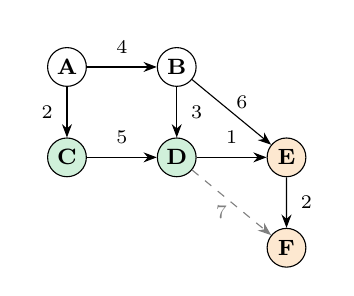
\begin{tikzpicture}[
  scale=0.82,
  every node/.style={circle,draw,minimum size=14pt,inner sep=1pt,font=\footnotesize\bfseries},
  lbl/.style={draw=none,fill=none,font=\scriptsize,inner sep=1pt},
  ->,>=Stealth]
  \node(A) at(0,0){A};
  \node(B) at(1.7,0){B};
  \node[fill=lightgreen](C) at(0,-1.4){C};
  \node[fill=lightgreen](D) at(1.7,-1.4){D};
  \node[fill=lightorange](E) at(3.4,-1.4){E};
  \node[fill=lightorange](F) at(3.4,-2.8){F};
  \draw(A)--node[lbl,above]{4}(B);
  \draw(A)--node[lbl,left]{2}(C);
  \draw(B)--node[lbl,right]{3}(D);
  \draw(B)--node[lbl,above right=-2pt]{6}(E);
  \draw(C)--node[lbl,above]{5}(D);
  \draw(D)--node[lbl,above]{1}(E);
  \draw(E)--node[lbl,right]{2}(F);
  \draw[dashed,gray](D)--node[lbl,below left=-2pt]{\color{gray}7}(F);
\end{tikzpicture}
\end{center}
\yb{\textbf{Clock rule:} start at 1; $+1$ each discover or finish. Gray=open. Black=finished.}

\cd{A(1)->B(2)->D(3)->E(4)->F(5)\\
F fin(6);E fin(7);D fin(8)\\
B->E: black->cross. B fin(9)\\
A->C(10)->D: black->cross\\
C fin(11); A fin(12)}

\begin{center}\scriptsize
\begin{tabular}{@{}cccl@{}}
\toprule
Node&disc&fin&Note\\\midrule
A&1&12&root, 1st tree\\
B&2&9&\\
D&3&8&\\
E&4&7&\\
F&5&6&leaf\\
C&10&11&root, 2nd tree\\\bottomrule
\end{tabular}
\end{center}

Tree edges: A$\to$B, B$\to$D, D$\to$E, E$\to$F, A$\to$C. Cross: B$\to$E, C$\to$D. No back edges $\Rightarrow$ DAG.

\gb{\textbf{Topo order} (decreasing fin): A(12)$\to$C(11)$\to$B(9)$\to$D(8)$\to$E(7)$\to$F(6) \checkmark}

\textbf{Kahn's}: remove in-degree-0 sources repeatedly. \textbf{Count orderings}: multiply \# sources at each step. Here always 1 $\Rightarrow$ unique.
\end{tcolorbox}

\vspace{3pt}
\begin{tcolorbox}[blue,title=DFS Edge Types]
\small
\begin{itemize}
  \item \textbf{Tree:} $v$ undiscovered when $(u,v)$ traversed
  \item \textbf{Back:} $v$ is ancestor (gray) $\Rightarrow$ \textbf{cycle!} $\Leftrightarrow$ not DAG
  \item \textbf{Forward:} $v$ descendant, already black
  \item \textbf{Cross:} $v$ black, different subtree
\end{itemize}
\yb{Undirected DFS: only tree + back edges. When $(u,v)$ seen and $v$ visited, $v$ must be ancestor since $(v,u)$ already explored.}
\end{tcolorbox}

\vspace{3pt}
\begin{tcolorbox}[purple,title=Graph T/F Traps]
\small
\gb{\textbf{TRUE:} $d(s,v)\leq R\;\forall v \Rightarrow d(u,v)\leq 2R$.\\ $d(u,v)\leq d(u,s)+d(s,v)\leq R{+}R{=}2R$ (triangle ineq.; undirected so $d(u,s)=d(s,u)$).}

\rb{\textbf{FALSE:} $|d(u)-d(v)|=1$ for all BFS edges. Counterex: triangle $s,u,v$ --- BFS gives $d(u)=d(v)=1$, edge $(u,v)$ gives 0. Correct: $\leq 1$.}

\rb{\textbf{FALSE:} SP stays SP in $G'$ (all weights $+1$). Counterex: 2-hop $1{+}1{=}2$ vs direct $2.5$; in $G'$: $4$ vs $3.5$ --- flipped. $k$-hop path gains $+k$; more hops penalized more.}
\end{tcolorbox}

\columnbreak

\begin{tcolorbox}[blue,title=Exercise 2a Graph (A--G) --- Official DFS]
\small
\textit{Edges: A$\to$B, A$\to$D, A$\to$F, B$\to$C, B$\to$D, C$\to$D, C$\to$E, E$\to$D, F$\to$G, G$\to$E. Alpha order from A.}
\begin{center}
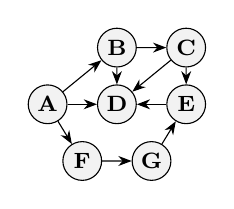
\begin{tikzpicture}[
  scale=0.8,
  every node/.style={circle,draw,fill=gray!10,minimum size=14pt,inner sep=0pt,font=\footnotesize\bfseries},
  ->,>=Stealth]
  \node(A) at(0,0){A};
  \node(B) at(1.1,0.9){B};
  \node(C) at(2.2,0.9){C};
  \node(D) at(1.1,0){D};
  \node(E) at(2.2,0){E};
  \node(F) at(0.55,-0.9){F};
  \node(G) at(1.65,-0.9){G};
  \draw(A)--(B);\draw(A)--(D);\draw(A)--(F);
  \draw(B)--(C);\draw(B)--(D);
  \draw(C)--(D);\draw(C)--(E);
  \draw(E)--(D);\draw(F)--(G);\draw(G)--(E);
\end{tikzpicture}
\end{center}
\gb{\textbf{disc/fin:} A(1/14) D(2/13) B(3/6) C(4/5) F(7/12) G(8/11) E(9/10)}

\cd{A(1)->B(2? No. A's alpha nbrs: B,D,F. Visits B(2)\\
->B: alpha nbrs C,D. C(3)->C fin(4? No: C->D,E.\\
C(3)->D(4)->D fin(5)->C fin(6)->B fin(7)? \\
Re-trace official: A(1)->D(2)->B(3)->C(4)\\
C fin(5)->B fin(6). D->F(7)->G(8)->E(9)\\
E fin(10)->G fin(11)->F fin(12)->D fin(13)->A fin(14)}

\yb{Official answer: A visits D \textit{second} (alpha: B then D), but then from D: B is unvisited, so D$\to$B first. Trace: A(1)$\to$D(2)$\to$B(3)$\to$C(4), C fin(5), B fin(6). Back to D$\to$F(7)$\to$G(8)$\to$E(9), E fin(10), G fin(11), F fin(12), D fin(13), A fin(14).}
\end{tcolorbox}

\vspace{3pt}
\begin{tcolorbox}[purple,title=Exercise 2c DAG --- Official Topo Sort]
\small
\textit{f$\to$c, f$\to$b, c$\to$a, c$\to$e, a$\to$h, a$\to$g, a$\to$d, b$\to$e, e$\to$g, g$\to$d}
\begin{center}
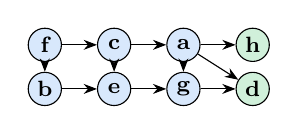
\begin{tikzpicture}[
  scale=0.8,
  every node/.style={circle,draw,fill=lightblue,minimum size=12pt,inner sep=0pt,font=\footnotesize\bfseries},
  ->,>=Stealth]
  \node(f) at(0,0.7){f};\node(c) at(1.1,0.7){c};
  \node(a) at(2.2,0.7){a};\node[fill=lightgreen](h) at(3.3,0.7){h};
  \node(b) at(0,0){b};\node(e) at(1.1,0){e};
  \node(g) at(2.2,0){g};\node[fill=lightgreen](d) at(3.3,0){d};
  \draw(f)--(c);\draw(c)--(a);\draw(a)--(h);
  \draw(f)--(b);\draw(b)--(e);\draw(e)--(g);\draw(g)--(d);
  \draw(c)--(e);\draw(a)--(g);\draw(a)--(d);
\end{tikzpicture}
\end{center}
\gb{\textbf{Official: f, c, a, h, b, e, g, d --- exactly 1 valid ordering.}}
\yb{Only f has in-degree 0. After removing f, only c has in-degree 0 (b still needs f's removal only, so b \textit{does} become available --- but c must precede a,e and the chain forces a unique order with no parallel choices.}
\end{tcolorbox}

\vspace{3pt}
\begin{tcolorbox}[purple,title=Exercise 2b --- Official SCC Construction]
\small
$V{=}\{s,a,b,c,d,e\}$, $E{=}\{(s,a),(a,b),(b,c),(c,d),(d,e),(e,b)\}$
\begin{center}
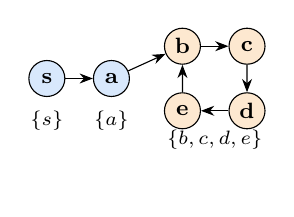
\begin{tikzpicture}[
  scale=0.82,
  every node/.style={circle,draw,minimum size=13pt,inner sep=0pt,font=\footnotesize\bfseries},
  ->,>=Stealth]
  \node[fill=lightblue](s) at(0,0){s};
  \node[fill=lightblue](a) at(1.0,0){a};
  \node[fill=lightorange](b) at(2.1, 0.5){b};
  \node[fill=lightorange](c) at(3.1, 0.5){c};
  \node[fill=lightorange](d) at(3.1,-0.5){d};
  \node[fill=lightorange](e) at(2.1,-0.5){e};
  \draw(s)--(a);\draw(a)--(b);\draw(b)--(c);
  \draw(c)--(d);\draw(d)--(e);\draw(e)--(b);
  \node[draw=none,fill=none,font=\scriptsize] at(0.0,-0.65){$\{s\}$};
  \node[draw=none,fill=none,font=\scriptsize] at(1.0,-0.65){$\{a\}$};
  \node[draw=none,fill=none,font=\scriptsize] at(2.6,-0.95){$\{b,c,d,e\}$};
\end{tikzpicture}
\end{center}
{\footnotesize Cycle b$\to$c$\to$d$\to$e$\to$b forms SCC$_3$. 6V, 6E. DFS from $s$ reaches all.\checkmark}

\textbf{Kosaraju}: (1) DFS on $G$, record fin order. (2) Reverse edges $\to G^R$. (3) DFS on $G^R$ in reverse fin order --- each tree $=$ one SCC. $O(V{+}E)$.
\end{tcolorbox}

\vspace{3pt}
\begin{tcolorbox}[purple,title=Connected Components]
\small
\kv{Undirected:}{BFS/DFS, count restarts $=$ \# components}
\kv{Directed weak:}{ignore directions, treat undirected}
\kv{Directed strong:}{Kosaraju $\Rightarrow$ SCCs}
\begin{itemize}
  \item No back edges in DFS $\Leftrightarrow$ DAG $\Leftrightarrow$ topo sort exists
  \item Condensation (SCC $\to$ node) always a DAG
  \item Undirected BFS: non-tree edges connect same/adjacent levels only
  \item SCC decomposition of any directed graph is unique
\end{itemize}
\end{tcolorbox}

\end{multicols}

\newpage

%%=============================================================
%% SIDE 2
%%=============================================================
\noindent{\centering\normalsize\bfseries\sffamily
  CS 3000 MIDTERM 2 --- SIDE 2: Shortest Paths, Dijkstra \& Problem Modeling\par}
\vspace{2pt}
\begin{multicols}{3}

\begin{tcolorbox}[teal,title=Dijkstra on Master Graph (source $A$)]
\small
\textit{A$\to$B(4), A$\to$C(2), B$\to$D(3), B$\to$E(6), C$\to$D(5), D$\to$E(1), E$\to$F(2), D$\to$F(7)}

\cd{Init: A=0 B=inf C=inf D=inf E=inf F=inf\\
Pop A(0): B->4, C->2\\
Pop C(2): D->2+5=7\\
Pop B(4): D->4+3=7(tie), E->10\\
Pop D(7): E->7+1=8*, F->7+7=14\\
Pop E(8): F->8+2=10*\\
Pop F(10): done.}

\begin{center}\scriptsize
\begin{tabular}{@{}cccc@{}}
\toprule Node&dist&via&Note\\\midrule
A&0&---&source\\
B&4&A&\\
C&2&A&popped 2nd\\
D&7&B or C&two equal paths\\
E&8&D&updated from 10\\
F&10&E&D$\to$F(14) beaten\\\bottomrule
\end{tabular}
\end{center}
\yb{\textbf{Once popped, dist is final.} Negative weights would let a popped node's dist improve later --- breaking this. Hence $w\geq 0$ required.}
\end{tcolorbox}

\vspace{3pt}
\begin{tcolorbox}[teal,title=Dijkstra --- Algorithm \& Runtimes]
\small
\cd{dist[s]=0; others inf\\
PQ = min-heap of all vertices\\
while PQ not empty:\\
\quad u = extract-min(PQ)\\
\quad for each neighbor v of u:\\
\quad\quad if dist[u]+w(u,v) < dist[v]:\\
\quad\quad\quad dist[v] = dist[u]+w(u,v)\\
\quad\quad\quad decrease-key(PQ,v,dist[v])}

\vspace{2pt}\textbf{Why correct}: when $u$ popped, all PQ nodes have dist $\geq$ dist$[u]$; non-negative weights mean no future edge can improve dist$[u]$.

\begin{center}\scriptsize
\begin{tabular}{@{}lll@{}}
\toprule PQ&Runtime&Use when\\\midrule
Array&$O(V^2)$&dense $E{=}\Theta(V^2)$\\
Bin heap&$O((V{+}E)\log V)$&general\\
Fib heap&$O(E{+}V\log V)$&very sparse\\\bottomrule
\end{tabular}
\end{center}
\rb{Requires $w\geq 0$. Negative weights $\Rightarrow$ Bellman-Ford $O(VE)$.}
\end{tcolorbox}

\vspace{3pt}
\begin{tcolorbox}[teal,title=Shortest Path Properties]
\small
\begin{itemize}
  \item \textbf{Subpath}: every subpath of a SP is a SP
  \item \textbf{Triangle ineq.}: $d(s,v)\leq d(s,u)+w(u,v)$
  \item \textbf{Relaxation}: if dist$[u]$ correct, relaxing $(u,v)$ gives correct SP through $u$
  \item \textbf{SP tree}: predecessor pointers form a spanning tree of SPs
\end{itemize}
\rb{\textbf{Adding $+c$}: $k$-hop path gains $+kc$. Different hop counts $\Rightarrow$ order can change $\Rightarrow$ SP not preserved.}
\gb{\textbf{Multiplying $\times c>0$}: all paths scale equally $\Rightarrow$ SP preserved.\checkmark}
\end{tcolorbox}

\vspace{3pt}
\begin{tcolorbox}[teal,title=BFS --- Algorithm \& Edge Property]
\small
\cd{BFS(G,s): d[s]=0; Q=[s]\\
while Q not empty:\\
\quad u = dequeue(Q)\\
\quad for each neighbor v of u:\\
\quad\quad if v not visited:\\
\quad\quad\quad d[v]=d[u]+1; enqueue(Q,v)}

\kv{Output:}{shortest hop-count paths from $s$}
\kv{Runtime:}{$O(V+E)$; Space: $O(V)$}
\yb{\textbf{Edge property:} $|d(u)-d(v)|\leq 1$ for any edge $(u,v)$ in undirected $G$.\\ \textit{Proof:} if $d(v)\geq d(u)+2$, when $u$ dequeued BFS would have set $d(v)=d(u)+1$ --- contradiction. Same-level edges give 0; $=1$ only for tree edges.}
\end{tcolorbox}

\columnbreak

\begin{tcolorbox}[amber,title=Exercise 4a --- Mario (Single Agent)]
\small
\kv{Vertices:}{$n$ islands}
\kv{Edges:}{directed; door $i$ from $u$ to $a_{u,i}$ with weight $w_{u,i}\geq 0$; $E=3n$}
\kv{Algorithm:}{Dijkstra from $s_1$ to $t$}
\kv{Runtime:}{$O(n\log n)$ time, $O(n)$ space \quad [$E=3n=O(n)$]}
\end{tcolorbox}

\vspace{3pt}
\begin{tcolorbox}[amber,title=Exercise 4b --- Mario + Luigi Synchronized]
\small
\textbf{Key insight}: model joint state as a single vertex.

\yb{\textbf{Vertices:} pairs $(u,v)$, $u$=Mario, $v$=Luigi. Up to $n^2$ nodes.\\[2pt]
\textbf{Edges:} $(u,v)\to(a_{u,i},a_{v,j})$ for all door pairs $(i,j)$.\\
\textbf{Weight:} $\max(w_{u,i},\,w_{v,j})$ --- slower agent is bottleneck.\\
$3{\times}3=9$ edges per node $\Rightarrow 9n^2$ edges total.\\[2pt]
\textbf{Source:} $(s_1,s_2)$ \quad \textbf{Target:} $(t,t)$\\
\textbf{Algorithm:} Dijkstra $\Rightarrow O(n^2\log n)$.}

\rb{\textbf{Why max?} Both move simultaneously each step; pair waits for the slower one.}
\rb{\textbf{Why Dijkstra?} $\max(w_{u,i},w_{v,j})\geq 0$ since all $w\geq 0$ --- non-negativity preserved.}
\end{tcolorbox}

\vspace{3pt}
\begin{tcolorbox}[amber,title=Exercise 5 --- Bikeways]
\small
\kv{Vertices:}{$t$ towns}
\kv{Edges:}{directed bikeways with $\ell(a)\leq L$ only}
\kv{Weights:}{$\ell(a)$ = length in miles}
\begin{enumerate}
  \item Keep only bikeways $\ell(a)\leq L$ \hfill$O(p)$
  \item Dijkstra from Centerville \hfill$O(p\log t)$
  \item Check all dist$[v]\leq M$ \hfill$O(t)$
\end{enumerate}
\gb{\textbf{Total: $O(p\log t)$} \quad (assumes $p\geq t$)}
\yb{\textbf{Why directed?} Bikeways one-way only. \textbf{Why filter first?} Bikeways $>{L}$ can never be used; removing before Dijkstra shrinks the graph.}
\end{tcolorbox}

\vspace{3pt}
\begin{tcolorbox}[red,title=Problem Modeling Checklist]
\small
\begin{enumerate}
  \item \textbf{States} $\to$ vertices (tuple for multi-agent)
  \item \textbf{Transitions} $\to$ edges (directed if asymmetric)
  \item \textbf{Costs} $\to$ weights (sum, max, etc.)
  \item \textbf{Constraints} $\to$ filter edges or restrict states
  \item \textbf{Goal} $\to$ source, target, algorithm
\end{enumerate}
\begin{center}\scriptsize
\begin{tabular}{@{}lll@{}}
\toprule Goal&Algorithm&Req.\\\midrule
SP $w\geq 0$&Dijkstra&$w\geq 0$\\
SP neg.&Bellman-Ford&no neg.\ cycle\\
Unweighted SP&BFS&---\\
Reachability&DFS/BFS&---\\
Topo order&DFS fin times&DAG\\
SCCs&Kosaraju&directed\\
All-pairs SP&Floyd-Warshall&no neg.\ cycle\\\bottomrule
\end{tabular}
\end{center}
\end{tcolorbox}

\columnbreak

\begin{tcolorbox}[red,title=Quick Runtimes]
\small
\begin{center}\scriptsize
\begin{tabular}{@{}lll@{}}
\toprule Algorithm&Time&Space\\\midrule
BFS/DFS&$O(V{+}E)$&$O(V)$\\
Topo sort&$O(V{+}E)$&$O(V)$\\
Kosaraju SCC&$O(V{+}E)$&$O(V)$\\
Dijkstra (array)&$O(V^2)$&$O(V)$\\
Dijkstra (heap)&$O((V{+}E)\log V)$&$O(V)$\\
Dijkstra (Fib)&$O(E{+}V\log V)$&$O(V)$\\
Bellman-Ford&$O(VE)$&$O(V)$\\
Floyd-Warshall&$O(V^3)$&$O(V^2)$\\\bottomrule
\end{tabular}
\end{center}
\kv{Dense:}{array Dijkstra $O(V^2)$}
\kv{Sparse $E{=}O(V)$:}{heap $\to O(V\log V)$}
\kv{Mario single:}{$O(n\log n)$}
\kv{Mario pair:}{$O(n^2\log n)$}
\kv{Bikeways:}{$O(p\log t)$}
\end{tcolorbox}

\vspace{3pt}
\begin{tcolorbox}[red,title=Greedy Proof Reference]
\small
\textbf{Stays ahead (induction):}
\begin{enumerate}
  \item Define measure; claim: $\forall\ell\leq k'$: greedy $\geq$ OPT
  \item Base $\ell{=}0$: trivial (same start)
  \item IH $\to$ step: local optimality maintains lead
  \item Conclude: $k'\leq k$
\end{enumerate}
\textbf{Exchange argument:}
\begin{enumerate}
  \item First diff index $i$: swap to greedy, cost $\not\uparrow$
  \item Repeat $\Rightarrow$ OPT $=$ greedy $\Rightarrow$ optimal
\end{enumerate}
\grb{GreedyJump uses stays-ahead (running distance measure), not exchange.}
\end{tcolorbox}

\vspace{3pt}
\begin{tcolorbox}[red,title=Common Mistakes]
\small
\rb{BFS: $|d(u)-d(v)|=1$ is \textbf{FALSE}. Same-level edges give 0. Correct: $\leq 1$.}
\rb{Weight $+c$: does NOT preserve SPs. $k$-hop path gains $+kc$; more hops penalized more.}
\rb{GreedyJump: inner loop overshoots (increments $j$ first), then appends $j-1$. Stone 0 always in output.}
\rb{Ex.\ 2a: official answer is D(disc=2). From A, alpha order is B,D,F --- visits B first, then from B visits C. Back to A: then D. But official trace shows A$\to$D(2). Verify directly with official solution.}
\yb{DFS: max fin $=2n$; disc $<$ fin always; no repeated fin times.}
\yb{SCC Ex.\ 2b: 4-node SCC is cycle b$\to$c$\to$d$\to$e$\to$b, not pairs with back-edges.}
\yb{GreedyJump: max avg jump IS optimized (3rd correct objective).}
\end{tcolorbox}

\vspace{3pt}
\begin{tcolorbox}[red,title=Exam Sanity Checks]
\small
\begin{itemize}
  \item DFS: max fin $=2n$; disc $<$ fin; no repeated times
  \item Topo: every edge goes left$\to$right in ordering
  \item Dijkstra: popped nodes never re-enter PQ; dist only decreases
  \item SCC: DAG $\Rightarrow$ each node own SCC; condensation always DAG
  \item BFS: $|d(u)-d(v)|\leq 1$ all edges; $=1$ only tree edges
  \item Runtime: state $V,E$ in problem terms before formula
  \item Graph model: confirm directed vs.\ undirected, $w\geq 0$ for Dijkstra
\end{itemize}
\end{tcolorbox}

\end{multicols}
\end{document}